\chapter{Introducción específica} % Main chapter title

\label{Chapter2}

%----------------------------------------------------------------------------------------
%	SECTION 1
%----------------------------------------------------------------------------------------
El objetivo de este capítulo es proporcionar una base teórica para comprender las herramientas y métodos utilizados en el desarrollo de este trabajo. En particular, se mencionarán las técnicas para el preprocesamiento de los datos, estrategias para el balanceo de clases, un repaso por los distintos modelos de inteligencia artificial y las métricas utilizadas para su evaluación. También se mencionarán conceptos básicos sobre plataformas de gestión de modelos de IA y servicios web.

\section{Tratamiento de los datos}

Una vez que se obtienen los datos para el entrenamiento de modelos de inteligencia artificial, es fundamental realizar un proceso de tratamiento de los datos para asegurar su calidad y adecuación para el análisis.
En primer lugar, la división de los datos en conjuntos de entrenamiento y prueba es una práctica común. Esto se hace para evaluar el rendimiento del modelo de manera efectiva, utilizando un conjunto de datos separado para el entrenamiento y otro para la evaluación, lo que ayuda a evitar el sobreajuste y a evaluar la capacidad de generalización del modelo.

Un punto clave en el tratamiento de datos es la corrección de valores inconsistentes o nulos. Esto implica identificar y corregir valores atípicos, faltantes o errores de entrada que podrían distorsionar el análisis y afectar la precisión del modelo. El valor faltante puede darse por diversas razones, como errores durante el ingreso manual de datos, mediciones incorrectas, fallas en el experimento, entre otras \citep{CAP2ARTICULO1}. Los valores faltantes son una realidad común en cualquier conjunto de datos y pueden tener un impacto significativo en el análisis y la interpretación de los resultados. Por lo tanto, es crucial entender las causas subyacentes y abordarlas adecuadamente durante el proceso de tratamiento de datos. Usualmente los datos faltantes se clasifican en los siguientes grupos: 
\begin{itemize}
\item Falta completamente al azar (MCAR): La probabilidad de que un registro tenga un valor faltante para un atributo no depende ni de los datos observados ni de los datos faltantes. Por ejemplo una muestra de laboratorio que se pierde.
\item Falta al azar (MAR): Indica que la probabilidad de que un registro tenga un valor faltante para un atributo podría depender de los datos observados, pero no del valor del dato faltante en sí mismo. Por ejemplo las personas con ingresos más altos pueden ser menos propensas a revelarlos en una encuesta, pero si la falta de respuesta es aleatoria dentro de las clases de ingresos, los datos de ingresos son faltantes al azar.
\item Falta no al azar (MNAR): Implica que la probabilidad de que un registro tenga un valor faltante para un atributo podría depender del valor del atributo mismo. Por ejemplo un sensor que no detecta temperaturas por debajo de cierto umbral, o personas que no completan los ingresos anuales en encuestas si superan cierto valor.
\end{itemize}

Para resolver el problema de los valores faltantes, existen diversos métodos de imputación de dichos valores. Estos son algunos de los más utilizados:
\begin{itemize}
\item Imputación por la media o mediana: Se remplazan los valores faltantes con la media o la mediana de la variable correspondiente. Esto es simple y rápido, pero puede introducir sesgos si la distribución de los datos es asimétrica o tiene valores atípicos.
\item Imputación por el valor más frecuente: Se remplazan los valores faltantes con el valor más común de la variable. Es útil para variables categóricas o variables con una distribución de frecuencia clara.
\item Imputación por regresión: Se utilizan modelos de regresión para predecir los valores faltantes a partir de las variables restantes. Esto puede ser más preciso que los métodos anteriores, pero puede ser computacionalmente intensivo y requiere asumir una relación lineal entre las variables.
\item Imputación por vecinos más cercanos (KNN): Los valores faltantes se estiman a partir de los valores de observaciones similares en el espacio de características. Este método puede ser efectivo en conjuntos de datos con estructuras de vecindario claras, pero puede ser sensible a la elección de la métrica de distancia y número de vecinos.
\item Imputación Múltiple por Ecuaciones Encadenadas (MICE): Se imputan los valores faltantes mediante la estimación secuencial de modelos predictivos, utilizando las variables restantes como predictores. Este método captura la incertidumbre asociada con la imputación de valores faltantes y puede proporcionar estimaciones más precisas.
\end{itemize}

Si los datos faltantes se consideran completamente aleatorios (MCAR), los métodos de imputación simples como la imputación por la media o mediana pueden ser apropiados. Cuando los datos faltantes son aleatorios (MAR), se pueden utilizar métodos más sofisticados como la imputación por regresión que utilizan información de otras variables observadas. Para datos no aleatorios (MNAR), la elección del método de imputación es más compleja y puede requerir técnicas específicas que modelen la relación entre los datos faltantes y los observados. Siempre es importante tener en cuenta las limitaciones y el contexto específico del conjunto de datos al tomar decisiones sobre el tratamiento de valores faltantes.

Otra de las técnicas que se pueden aplicar a los datos es la discretización, que es la conversión de variables continuas en variables discretas o categóricas. Esta técnica ayuda a que los modelos generen reglas mas breves y comprensibles, reduciendo la complejidad, y también es útil para aumentar la generalización y precisión del conocimiento \citep{CAP2ARTICULO2}.

Y por último, para obtener un conjunto de datos completamente numérico, se suele utilizar la codificación de variables categóricas. Esta técnica incluye métodos como la codificación \textit{one-hot} que convierte las variables categóricas en representaciones numéricas, asignando un valor binario a cada categoría. Además existen otras técnicas de codificación, como la codificación de etiquetas (\textit{label encoding}) y la codificación de frecuencia (\textit{frequency encoding}), que también se utilizan para transformar variables categóricas en datos numéricos compatibles con algoritmos de aprendizaje automático \citep{CAP2ARTICULO3}.

Las técnicas anteriormente mencionadas proveen soluciones a los problemas que suelen encontrarse en los conjuntos de datos y ayudan a garantizar la calidad y la adecuación para su posterior análisis y entrenamiento de modelos.


\section{Desbalance de clases}

El desbalance de clases es un problema común en el aprendizaje automático, donde una o más clases están subrepresentadas en comparación con otras en el conjunto de datos \citep{CAP2ARTICULO4}. Esto puede ser problemático porque los algoritmos de aprendizaje automático tienden a favorecer las clases mayoritarias y pueden tener dificultades para aprender patrones en las clases minoritarias.
El desbalance de clases puede llevar a modelos sesgados y poco precisos, especialmente en problemas de clasificación donde la precisión de las clases minoritarias es de particular interés, como la detección de fraudes, enfermedades o anomalías.

Algunas técnicas comunes para abordar el desbalance de clases incluyen:
\begin{itemize}
\item Submuestreo: Se reduce el número de muestras de las clases mayoritarias para equilibrar la proporción de clases. Esto puede ayudar a prevenir el sesgo hacia las clases mayoritarias, pero también puede resultar en la pérdida de información valiosa.
\item Sobremuestreo: Implica aumentar el número de muestras de las clases minoritarias mediante técnicas como la replicación de instancias o la generación de nuevas muestras sintéticas. Esto puede ayudar a mejorar la representación de las clases minoritarias y a evitar el sesgo hacia las clases mayoritarias.
\item Ponderación de clases: Algunos algoritmos de aprendizaje automático permiten asignar pesos diferentes a las clases para tener en cuenta el desbalance de clases durante el entrenamiento del modelo. Esto puede ayudar a compensar la falta de representación de las clases minoritarias.
\end{itemize}

En la figura \ref{fig:diagDesbalance} se muestra la diferencia entre las técnicas de submuestreo y sobremuestreo.

\begin{figure}[htpb]
\centering 
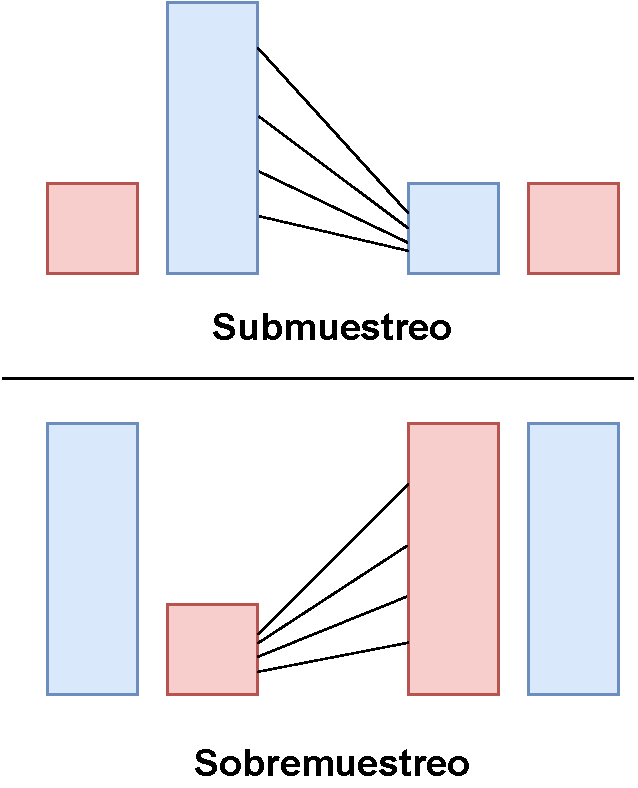
\includegraphics[width=.55\textwidth]{./Figures/Desbalance.pdf}
\caption{Submuestreo y sobremuestreo.}
\label{fig:diagDesbalance}
\end{figure}

Para el caso de submuestreo, existen varias técnicas utilizadas para equilibrar el desbalance de clases. Una de ellas es el submuestreo aleatorio (\textit{Random Undersampling}), donde se eliminan aleatoriamente un subconjunto de muestras de la clase mayoritaria para igualar el número de muestras de la clase minoritaria. Otra técnica es la de muestras cercanas (\textit{NearMiss}), que elimina muestras de la clase mayoritaria que están próximas a las muestras de la clase minoritaria en el espacio de características, preservando así la información relevante.

En cuanto al sobremuestreo, se puede aplicar la técnica de duplicación de muestras aleatorias (\textit{Random Oversampling}), que consiste en duplicar las muestras de la clase minoritaria para aumentar su representación en el conjunto de datos. Pero también existen técnicas para la generación de muestras sintéticas, como SMOTE (\textit{Synthetic Minority Over-sampling Technique}), que crea nuevas muestras interpoladas entre las muestras existentes de la clase minoritaria, lo que ayuda a mejorar su representación sin duplicar directamente las muestras existentes. 

Cada técnica tiene sus ventajas y desventajas y muchas veces se usa una combinación de ellas. La elección adecuada depende del conjunto de datos específico y del problema en cuestión. Es importante experimentar con diferentes enfoques y evaluar su rendimiento para determinar la estrategia más efectiva.


\section{Modelos de inteligencia artificial}

Los modelos de inteligencia artificial son comúnmente utilizados para reconocer patrones en grandes conjuntos de datos y obtener predicciones. Se dice que los modelos aprenden cuando logran mejorar sus resultados en una tarea específica luego de procesar muchos datos y sin obtener instrucciones explicitas de un programador \citep{ARTICULO2}. 
Los tipos de aprendizaje se dividen en los siguientes tres:
\begin{itemize}
\item Aprendizaje supervisado: Para entrenar al modelo se utiliza un conjunto de datos etiquetados. Esto quiere decir que se le provee tanto las características como el valor objetivo esperado. El modelo aprende a hacer predicciones basadas en estos ejemplos y se ajusta para minimizar los errores entre las predicciones y las etiquetas conocidas.
\item Aprendizaje no supervisado: No se utilizan etiquetas en los datos de entrenamiento. El modelo explora patrones y estructuras en los datos sin una guía explícita. Este enfoque es útil cuando no conocemos las categorías de antemano y queremos descubrir patrones ocultos.
\item Aprendizaje por refuerzo: El modelo aprende a tomar decisiones a través de la interacción con un entorno. Para cada acción recibirá recompensas o castigos según su desempeño. El objetivo es maximizar las recompensas a lo largo del tiempo.
\end{itemize}

Teniendo los datos y el tipo de aprendizaje que se desea implementar, se debe buscar también una arquitectura de modelo que tenga la capacidad de aprender de los datos y devolver predicciones. 
Dentro de la inteligencia artificial, existe un universo que se conoce como \textit{Machine Learning} (ML) o aprendizaje automático, que refiere a aquellos algoritmos que utilizan métodos estadísticos para analizar datos, aprender de ellos y elaborar predicciones o sugerencias. Entre los modelos de ML mas conocidos se encuentran los siguientes:

\begin{itemize}
\item Regresión Lineal: Se utiliza para predecir valores continuos basados en variables independientes. Busca la relación lineal entre las variables de entrada y salida.
\item Regresión Logística: Se utiliza para clasificación binaria. Estima la probabilidad de que una instancia pertenezca a una determinada clase.
\item Árboles de Decisión: Organizan las características de los datos en una estructura similar a un árbol. Cada nodo en este árbol representa una pregunta sobre una característica específica de los datos. Por ejemplo, podría ser ¿Tiene diabetes? o ¿Es menor de 30 años?. Las ramas del árbol representan las posibles respuestas a estas preguntas, como sí o no. Siguiendo las ramas del árbol, eventualmente se llega a una hoja que representa la decisión o predicción final.
\item Random Forest: Es una técnica de conjunto que combina múltiples árboles de decisión. Cada árbol se entrena con una muestra aleatoria del conjunto de datos y luego las predicciones se promedian para obtener la salida final.
\item Support Vector Machine (SVM): Es un algoritmo de clasificación que encuentra el hiperplano óptimo que mejor separa las clases en un espacio de características de alta dimensión. Puede ser usado tanto para clasificación como para regresión.
\end{itemize}

Dentro del universo ML, hay otro grupo mas chico que se denomina \textit{Deep Learning} (DL) o aprendizaje profundo, en donde los algoritmos utilizan una arquitectura de redes neuronales que simulan el comportamiento del cerebro humano, por lo que suelen ser mucho mas grandes y complejos.
Estos últimos suelen usarse para tareas de visión por computadora o procesamiento de lenguaje natural, y requieren mucha potencia de cómputo y grandes cantidades de datos.
En la figura \ref{fig:diagMLvsDL} se puede visualizar la diferencia entre utilizar modelos de \textit{Machine Learning} y modelos de \textit{Deep Learning} para obtener predicciones.

\begin{figure}[htpb]
\centering 
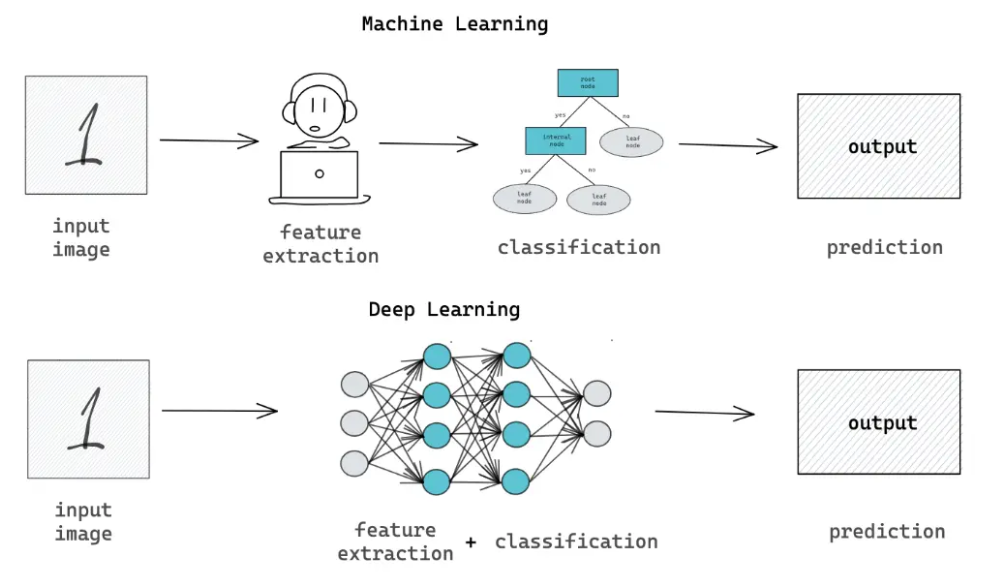
\includegraphics[width=.95\textwidth]{./Figures/ML vs DL.png}
\caption{Machine Learning vs Deep Learning.}
\label{fig:diagMLvsDL}
\end{figure}

Los modelos también se diferencian por el tipo de predicción que realizan. Un modelo que predice un valor continuo, como el precio de una vivienda, se lo conoce como modelo de regresión. Mientras que a un modelo que predice una etiqueta o clase, ya sea binaria o multi-clase, se lo conoce como modelo de clasificación. 

Este último tipo de modelo es muy utilizado en medicina, ya que sirve para predecir la presencia o ausencia de cierta enfermedad, o para predecir su tipo específico.
En este trabajo en particular, se utilizaron modelos de clasificación con aprendizaje supervisado. Se usaron arquitecturas de modelos de \textit{Machine Learning} y de \textit{Deep Learning} con el propósito de predecir el riesgo de mortalidad de pacientes en diálisis renal. Es importante señalar que se trata de una clasificación binaria puesto que la variable objetivo tiene dos posibles valores: no hay riesgo ("0") o hay riesgo ("1") de mortalidad.

\section{Evaluación de modelos de clasificación}

Para evaluar el comportamiento de un modelo de clasificación binaria comúnmente se recurre a una herramienta llamada matriz de confusión. Esta matriz, como se muestra en la figura \ref{fig:MatrizConfusion}, presenta las clases predichas en las columnas y las clases reales en las filas. A partir de esta tabla, se derivan cuatro métricas clave:

\begin{figure}[htpb]
\centering 
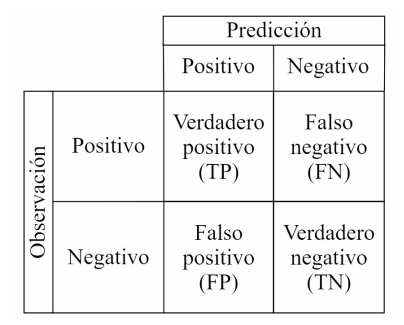
\includegraphics[width=.75\textwidth]{./Figures/MatrizDeConfusion.png}
\caption{Matriz de confusión.}
\label{fig:MatrizConfusion}
\end{figure}

\begin{itemize}
\item Verdaderos positivos (TP): Representan las predicciones correctas de una condición positiva.
\item Verdaderos negativos (TN): Son las predicciones correctas de una condición negativa.
\item Falsos positivos (FP): Se dan cuando el modelo predice incorrectamente una condición positiva que en realidad no lo es.
\item Falsos negativos (FN): Se dan cuando el modelo predice incorrectamente la ausencia de una condición positiva que en realidad está presente.
\end{itemize}

En contextos médicos, los falsos negativos pueden tener consecuencias significativas para la salud del paciente, ya que se está prediciendo que un paciente no tiene cierta condición cuando en realidad la tiene. 

Particularmente en este trabajo, los falsos negativos podrían implicar no tomar medidas necesarias para un tratamiento adecuado, aumentando el riesgo de mortalidad del paciente. Por lo tanto, es fundamental minimizar la tasa de falsos negativos tanto como sea posible, incluso si esto conlleva un aumento en los falsos positivos. 

Derivados de estos 4 valores de la matriz de confusión se definen las siguientes métricas para evaluar el rendimiento de un modelo de clasificación:

\begin{itemize}
\item \textit{Precision}: Es la proporción de ejemplos positivos que fueron correctamente clasificados como positivos respecto al total de ejemplos clasificados como positivos. Es decir, mide la calidad de las predicciones positivas del modelo. Se calcula como TP / (TP + FP).
\item \textit{Recall}: Es la proporción de ejemplos positivos que fueron correctamente clasificados como positivos respecto al total de ejemplos que son realmente positivos. Es decir, mide la capacidad del modelo para encontrar todos los ejemplos positivos. Se calcula como TP / (TP + FN).
\item \textit{F1 Score}: Es la media armónica de la \textit{precision} y el \textit{recall}. Proporciona un equilibrio entre ambas métricas y es útil cuando hay un desequilibrio entre las clases. Se calcula como 2 * (\textit{precision} * \textit{recall}) / (\textit{precision} + \textit{recall}).
\item \textit{Accuracy}: Es la proporción de ejemplos clasificados correctamente (tanto positivos como negativos) respecto al total de ejemplos. Es una métrica general de la calidad del modelo en todas las clases. Se calcula como (TP + TN) / (TP + TN + FP + FN).
\item AUC (\textit{Area Under the Curve}): El AUC es el área bajo la curva ROC (\textit{Receiver Operating Characteristic}). La curva ROC es una representación gráfica de la sensibilidad frente a la tasa de falsos positivos para diferentes umbrales de clasificación. El AUC mide la capacidad del modelo para distinguir entre clases positivas y negativas. Un valor de AUC cercano a 1 indica un buen rendimiento del modelo, mientras que un valor cercano a 0.5 indica un rendimiento aleatorio.
\end{itemize}

En este trabajo se utilizaron las métricas antes mencionadas para la evaluación de los modelos entrenados, prestando especial atención a las métricas de \textit{F1 Score} y \textit{Recall}, ya que existe un desbalance entre las clases y es importante detectar correctamente a la mayoría de casos positivos.

\section{Plataforma de gestión de modelos}

Una plataforma de gestión de modelos de IA es una herramienta diseñada para ayudar a los equipos de desarrollo y científicos de datos a gestionar, monitorear y desplegar modelos de manera eficiente. Estas plataformas ofrecen las siguientes ventajas:

\begin{itemize}
\item Centralización: Permiten centralizar todos los modelos en un único lugar, facilitando su gestión y acceso.
\item Implementación automatizada: Facilitan la implementación de modelos en entornos de producción, proporcionando herramientas para la integración continua y la implementación continua (CI/CD).
\item Versionado: Ofrecen capacidades de versionado para los modelos, lo que facilita el seguimiento de cambios y la colaboración entre equipos.
\end{itemize}

Existen múltiples plataformas para gestión de modelos \textit{Open Source}, tales como MLFlow, Apache Airflow o Jenkins, las cuales se conectan directamente con repositorios en la nube, como GitHub, y descargan modelos para aplicar en distintos ambientes. También cuentan con la posibilidad de realizar re-ntrenamientos automáticos de los modelos cuando se cuente con nuevos conjuntos de datos, aunque este punto queda fuera del alcance de este trabajo. En este trabajo se configura Jenkins como plataforma de gestión de modelos.

\section{Servicios Web}

Una vez que el modelo de IA fue entrenado y desplegado en un algún ambiente, el siguiente paso es exponerlo a través de un servicio web. Esto generalmente se logra mediante la creación de una API (\textit{Application Programming Interface}).
Comúnmente se utilizan APIs para la interacción entre diferentes sistemas informáticos, facilitando el intercambio de datos y la ejecución de funciones remotas. Se suele utilizar también para el desarrollo de aplicaciones web y móviles, para solicitar datos de alguna fuente de información como una base de datos.
Se caracterizan por estar estructurados con métodos que requieren parámetros específicos y proporcionan respuestas predefinidas, lo que simplifica la interacción entre sistemas. Esta estandarización les otorga independencia de plataforma y lenguaje, lo que los convierte en herramientas altamente adaptables y versátiles.

En esta caso, la API actúa como un intermediario entre la aplicación cliente y el modelo de IA, facilitando la comunicación y la interacción. Como primer paso, recibe los datos del cliente en un formato especificado y realiza el pre-procesamiento de los mismos, tal como se realizó durante el entrenamiento del modelo. Una vez procesados los datos se realiza la consulta al modelo de IA para obtener una predicción como respuesta. Dicha predicción es la que se devuelve al cliente como respuesta del llamado a la API.

En este trabajo se desarrolla una API para el acceso al modelo que contiene métodos para obtener predicciones individuales o masivas. También se desarrolla una aplicación cliente que llama automáticamente a la API cada cierto período de tiempo para solicitar predicciones y genera reportes para el usuario final.